\newpage
\subsection[Architektur]{Architektur \label{sec:Architektur}
 \\ \textnormal{\small{\textit {Verfasst von Melanie Hammerschmidt}}}}
 
Die Applikation ist streng nach dem Konzept des Model-View-Controller aufgebaut.
\\
Model-View-Controller ist ein Design Pattern, das vielleicht am häufigsten verwendete Muster, welches für heutige Programmierung eingesetzt wird \cite{MVC}. Es setzt eine strikte Trennung von Teilkomponenten voraus, die für eine hohe Wiederverwendbarkeit und einen strukturierten Aufbau sorgen. Im Falle einer GUI-Anwendung trennt man bei Anwendung dieses Patter das Model, die View und den Controller. Das Pattern ist also lediglich eine Erweiterung der schon seit langem verbreiteten Trennung von Eingabe (Controller), Verarbeitung (Model) und Ausgabe (View). 

\begin{figure}[h]
\centering
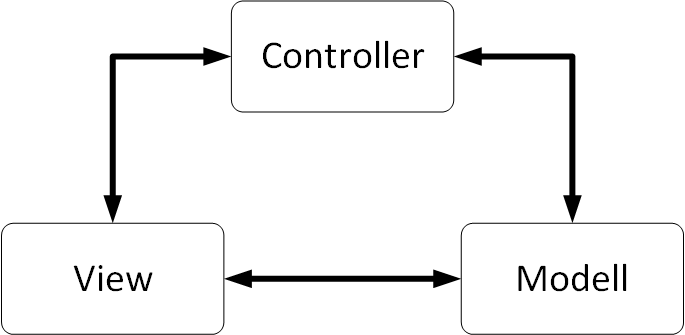
\includegraphics[width=0.4\textwidth]{ref/images/mvc.png}
\caption[Modell-View-Controller Pattern]{Modell-View-Controller Pattern}
\label{fig:MVC}
\end{figure} 

Das Model sorgt sich dabei allein um die Verarbeitung der Daten einer Anwendung. Alle Änderungen, die an den Daten ausgeführt werden sollen, finden im Model statt. Ein Model kann mit beliebig vielen Views verbunden werden und so Informationen austauschen. 
\\
Eine View kümmert sich um die graphische Darstellung der Anwendungsdaten, die es von seinem konkret zugewiesenen Model erhält. 
\\
Der Controller ist für die Möglichkeiten des Anwendungsnutzers zur Interaktion zuständig. Er übernimmt die Zuordnung von Benutzereingaben zu Funktionen des Models. Um diese Überleitung zu ermöglichen müssen sowohl Verbindungen zu Models als auch zu den Views existieren.
\\
Entsprechend dieses Patterns ist die Architektur der hier beschriebenen Applikation ebenfalls strukturiert gehalten. Einfach gesagt, besteht die Applikation lediglich aus einer HTML-Seite, die immer wieder mit verändertem Inhalt dargestellt wird. Diese wird mithilfe von Javascript (Angular JS) ständig mit dem Inhalt einer neuen View gefüllt.
\\
Für jede dargestellte Seite der Applikation existiert eine View. Diese besteht ebenfalls wieder aus einer einfache HTML-Seite, die allerdings über einen extra dafür definierten Controller mittels Variablen- und Funktionszuweisung verändert werden kann. Dieser Controller weißt auch die Methoden, die dann z.B. bei einem Button-Druck ausgeführt werden können, die entsprechende Verarbeitung zu.
\\
Diese Verarbeitung findet in sogenannten Services statt. In jedem Controller besteht die Möglichkeit auf diese Services zuzugreifen. Sie bilden das Model in unserer Model-View-Controller-Darstellung. Sie enthalten die Daten und können sich sowohl mit dem lokalen Speicher des genutzten Geräts als auch mit dessen spezifischen Daten verbinden. Außerdem können an dieser Stelle auch selbst definierte Werte und damit verbundene Funktionen hinterlegt werden, die jeder Controller aufrufen kann.
\\
Um zwischen den einzelnen View wechseln zu können, wird immer ein aktueller Status der Applikation gespeichert. Dieser Status entscheidet, welche View und welcher dazugehörige Controller in dem Moment verwendet werden. Über den Status der Applikation kann man ganz leicht zwischen den Views unterscheiden und jeder Status hat seinen eigenen Historienstapel. Dadurch lassen sich vergangene Klicks des Anwenders leicht rückgängig machen.
\\
Allgemein kann man zwei verschiedene Prozess-Ablaufarten unterscheiden. 
\begin{figure}[h]
\centering
\includegraphics[width=0.9\textwidth]{ref/images/mvc-ablauf.png}
\caption[Ablauf der Modell-View-Controller]{Ablauf der Modell-View-Controller}
\label{fig:MVC-Ablauf}
\end{figure} 

Die View kann Daten zur Anzeige anfordern, die sie selbst nicht besorgen kann (Datenaufbereitung) oder der Nutzer aktiviert z.B. durch Klick auf einen Button eine Funktion, die der Controller (bzw. dann der Service) anbietet (Funktionsdurchführung).